\documentclass[../review_3.tex]{subfiles}
\graphicspath{{\subfix{../img/}}}
\begin{document}

\chapter{Überprüfung der Anforderungen}\thispagestyle{fancy}

In diesem Kapitel wird geklärt, in wie fern das entwickelte System den zu Beginn des Projekts aufgestellten funktionalen und nichtfunktionalen Anforderungen gerecht wird. Dafür wird zunächst kurz auf deren Priorisierung eingangen. Anschließend werden die Anforderungen aufgelistet und kurz erklärt, ob diese erfüllt worden sind oder nicht.
\vspace{-0.2cm}
\section{Priorisierung der Anforderungen}\thispagestyle{fancy}
Um Anforderungen zu strukturieren und nach Wichtigkeit zu priorisieren, wird in der Regel ein System zur Klassifizierung der Eigenschaften verwendet. Hier wurde eine Priorisierung nach der \textbf{MuSCoW}-Methode vorgenommen:
\begin{description}
    \item{\textbf{Must}:} Diese Anforderungen sind unbedingt erforderlich und nicht verhandelbar. Sie sind erfolgskritisch für das Projekt.
    \item{\textbf{Should}:} Diese Anforderungen sollten umgesetzt werden, wenn alle Must-Anforderungen trotzdem erfüllt werden können.
    \item{\textbf{Could}:} Diese Anforderungen können umgesetzt werden, wenn die Must- und Should-Anforderungen nicht beeinträchtigt werden. Sie haben geringe Relevanz und sind eher ein \glqq Nice to have\grqq.
    \item{\textbf{Won't}:} Diese Anforderungen werden im Projekt explizit nicht umgesetzt, werden aber eventuell für die Zukunft vorgemerkt.
\end{description}

\vspace{-0.2cm}

\section{Funktionale Anforderungen}

Die funktionalen und die nichtfunktionalen Anforderungen werden in einzelnen Unterkapiteln getrennt behandelt. Für beide Arten wird zunächst die Tabelle aus dem Pflichtenheft erneut dargestellt. Nach der Auflistung wird eine Überprüfung zum einen anhand des Testdrehbuch und nach anderen Methoden vorgenommen.

\subsection{Auflistung der funktionalen Anforderungen}
% Sie beschreiben das Systemverhalten durch Spezifikation der erwarteten Input-/Output-Beziehungen
% --> Was soll umgesetzt werden?

Funktionale Anforderungen legen konkret fest, was das System können soll. Hier wird unter anderem beschrieben, welche Funktionen das System bieten soll. Die folgende Tabelle zeigt diese funktionalen Anforderungen.

\begin{longtable} [h] {p{1cm} p{4cm} p{7cm} l}
   \toprule
   \textbf{ID}                                                                                                                                                                                                      & \textbf{Name}                                  & \textbf{Beschreibung}                                                                                                                                                                                                                                   & \textbf{MuSCoW} \\ \midrule \endhead
    F01                                                                                                                                                                                                              & Lokale Administration                          & Das System muss lokal per Command-Line-Interface administriert werden können.                                                                                                                                                                           & Must            \\
    F02                                                                                                                                                                                                              & Angriffsarten                                  & Das System muss die Folgen der aufgelisteten (D)DoS-Angriffe abmildern können: \begin{itemize} \setlength{\parskip}{-2pt}
        \item SYN-Flood
        \item SYN-FIN Attack
        \item SYN-FIN-ACK Attack
        \item TCP-Small-Window Attack
        \item TCP-Zero-Window Attack
        \item UDP-Flood
    \end{itemize}
    Dabei ist vorausgesetzt, dass das Ziel eines Angriffes eine einzelne Station in einem Netzwerk ist und kein Netzwerk von Stationen. Es sind also direkte Angriffe auf einzelne Server, Router, PC, etc. gemeint. & Must                                                                                                                                                                                                                                                                                                                       \\
    F03                                                                                                                                                                                                              & Keine zusätzliche Angriffsfläche               & Besonders darf das System den unter ,,Angriffsarten'' spezifizierten Angriffen keine zusätzliche Angriffsfläche bieten, d.h. es darf es auch nicht durch Kenntnis der Implementierungsdetails möglich sein, das System mit diesen Angriffen zu umgehen. & Must            \\
    F04                                                                                                                                                                                                              & L3/ L4 Protokolle                              & Das System muss mit gängigen L3/L4 Protokollen klarkommen.                                                                                                                                                                                             & Must            \\
    F05                                                                                                                                                                                                              & Modi                                           & Passend zum festgestellten Angriffsmuster muss das System eine passende Abwehrstrategie auswählen und ausführen.                                                                                                                                        & Must            \\
    F06                                                                                                                                                                                                              & Position                                       & Das System soll zwischen dem Internet-Uplink und dem zu schützenden System oder einer Menge von Systemen platziert werden.                                                                                                                              & Must            \\
    F07                                                                                                                                                                                                              & Weiterleiten von Paketen                       & Das System muss legitime Pakete vom externen Netz zum Zielsystem weiterleiten können.                                                                                                                                                                   & Must            \\
    F08                                                                                                                                                                                                              & Installation und Deinstallation                & Das System muss durch Befehle in der Kommandozeile zu installieren und zu deinstallieren sein. Hilfsmittel hierzu sind: Installationsanleitung, Installationsskript, Meson und Ninja.                                                                   & Must            \\
    F09                                                                                                                                                                                                              & Mehrere Angriffe nacheinander und zeitgleich & Das System muss mehreren Angriffen nacheinander und zeitgleich standhalten, hierbei muss berücksichtigt werden, dass auch verschiedene Angriffsarten und Muster zur gleichen Zeit erkannt und abgewehrt werden müssen.                                  & Must            \\
    F10
    
    & IPv4                                           & Das System muss mit IPv4-Verkehr zurechtkommen.                                                                                                                                                                                                         & Must            \\
    F11                                                                                                                                                                                                                                                                                            & Hardware                                       & Das System soll nicht Geräte- bzw. Rechnerspezifisch sein.                                                                                                                                                                                              & Should          \\
    F12                                                                                                                                                                                                              & Zugriff                                        & Der Zugriff auf das lokale System soll per SSH oder Ähnlichem erfolgen, um eine Konfiguration ohne Monitor zu ermöglichen.                                                                                                                              & Should          \\
    F13                                                                                                                                                                                                              & Betrieb                                        & Das System soll auf Dauerbetrieb ohne Neustart ausgelegt sein.                                                                                                                                                                                          & Should          \\
    F14                                                                                                                                                                                                              & Privacy                                        & Das System soll keine Informationen aus der Nutzlast der ihm übergebenen Pakete lesen oder verändern.                                                                                                                                                   & Should          \\
    F15                                                                                                                                                                                                              & Konfiguration                                  & Der Administrator soll die Konfiguration mittels Konfigurationsdateien ändern können.                                                                                                                                                                   & Can             \\
    F16                                                                                                                                                                                                              & Abrufen der Statistik                          & Der Administrator soll Statistiken über das Verhalten des Systems abrufen können.                                                                                                                                                                       & Can             \\
    F17                                                                                                                                                                                                              & Starten und Stoppen des Systems                & Der Administrator soll das System starten und stoppen können.                                                                                                                                                                                           & Can             \\
    F18                                                                                                                                                                                                              & Informieren des Anwenders                      & Der Anwender soll über Angriffe informiert werden.                                                                                                                                                                                                      & Can             \\
    F19                                                                                                                                                                                                              & Administration über graphische Oberfläche      & Das System soll über eine graphische Oberfläche administriert werden können.                                                                                                                                                                            & Can             \\
    F20                                                                                                                                                                                                              & IPv6                                           & Das System soll mit IPv6-Verkehr zurechtkommen können                                                                                                                                                                                                   & Can             \\
    F21                                                                                                                                                                                                              & Weitere Angriffsarten                          &  Das System schützt weder vor anderen außer den genannten DoS-Angriffen (siehe F02 \glqq Angriffsarten\grqq)-insbesondere nicht vor denjenigen, welche auf Anwendungsebene agieren-, noch vor anderen Arten von Cyber-Attacken, die nicht mit DoS in Verbindung stehen.
    So bleibt ein Intrusion Detection System weiterhin unerlässlich.                                                                            & Won't           \\
    F22                                                                                                                                                                                                              & Anzahl der zu schützenden Systeme              & Das System wird nicht mehr als einen Server, Router, PC, etc. vor Angriffen schützen.                                                                                                                                                                   & Won't           \\
    F23                                                                                                                                                                                                              & Fehler des Benutzers                           & Das System soll nicht vor Fehlern geschützt sein, da es durch eine nutzungsberechtigte Person am System ausgeführt wird.  So sollen beispielsweise Gefährdungen, welche aus fahrlässigem Umgang des Administrators mit sicherheitsrelevanten Softwareupdates resultieren, durch das zu entwickelnde System nicht abgewehrt werden.                                                                                                                              & Won't           \\
    F24                                                                                                                                                                                                              & Softwareupdates                                & Das System soll keine Softwareupdates erhalten und soll nicht gewartet werden.                                                                                                                                                                                      & Won't           \\
    F25                                                                                                                                                                                                              & Router-/Firewall-Ersatz                                & Das System soll  nicht als Router oder als Firewall-Ersatz verwendet werden.                                                                                                   & Won't           \\
    F26                                                                                                                                                                                                              & Hardware-Ausfälle                              & Das System soll keine Hardwareausfälle (zum Beispiel auf den Links) beheben.                                             & Won't           \\
    F27                                                                                                                                                                                                              & Fehler in Fremdsoftware                              & Das System kann nicht den Schutz des Servers bei Fehlern in Fremdsoftware garantieren.    & Won't        \\ \bottomrule
\end{longtable} %fehlt: Pakete weiterleiten, Pakete verwerfen

\subsection{Überprüfung der funktionalen Anforderungen}
Jede einzelne funktionale Anforderungen wird hier in einem kleinen Unterkapitel überprüft. Die Reihenfolge ist dabei die gleiche wie in der oben stehenden Tabelle.

\subsubsection{F01: Lokale Administration}
Diese Muss-Anforderung wurde erfüllt. Ein Command-Line-Interace wurde mithilfe von Konventionen wie \glqq Human first design\grqq{} erstellt. So soll es beispielsweise den Nutzer nicht mit für Menschen irrelevanten Informationen überschütten und vorschlagen, was als Nächstes gemacht werden kann.

Mit Hilfe der Kommandos \texttt{help} oder \texttt{h} bekommt der Nutzer alle gültigen Eingaben angezeigt. Bei einer ungültigen Eingabe wird auf diesen Hilfsbefehl verwiesen. Die Eingabe von \texttt{exit} beendet das Programm, sodass zur normalen Kommandozeile zurückgekehrt wird. Der nachfolgende Bildschirmausschnitt (vgl. Abb \ref{cli}) zeigt diese Funktionen beispielhaft.

\begin{figure} [h]
    \centering
    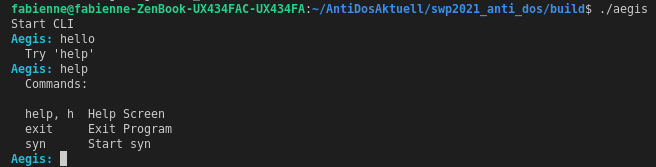
\includegraphics[width = \linewidth, trim=0pt 0pt 0pt 2pt, clip]{img/CLIAegis.png}
    \caption{Screenshot des CLIs von Aegis}
    \label{cli}
\end{figure}

%Cli Attacker

\subsubsection{F02: Angriffsarten}
% Test Nr. 6 (Überprüfung Widerstandsfähigkeit der Miditation-Box)
% Das System muss die Folgen der aufgelisteten (D)DoS-Angriffe abmildern können:
AEGIS ist in der Lage folgende Angriffe vollständig abzuwehren:
\begin{itemize}
    \setlength{\parskip}{-2pt}
    \item SYN-FIN Attack,
    \item SYN-FIN-ACK Attack, 
    \item SYN-Flood
\end{itemize}

Nach Integration des bereits implementierten Pakets \texttt{Inspection} wäre AEGIS in der Lage folgende Angriffe abzumildern: 
\begin{itemize}
    \setlength{\parskip}{-2pt}
    \item UDP-Flood, 
    %\item ICMP-Flood,
    \item Zero-Window, 
    \item Small-Window
\end{itemize}

Es wird von abmildern geschrieben, da es legitime Pakete geben kann, die die sieben Charakteristiken besitzen wie Angriffspakete. Dementsprechend ist es notwendig ,eine gewisse Menge dieser Pakete zu tolerieren.
Allerdings wurde das Modul zur Abwehr letzterer Angriffe, zum Zeitpunkt der Niederschrift, noch nicht integriert.

\subsubsection{F03: Keine zusätzliche Angriffsfläche}
% Test Nr. 4 (Überprüfung Abwehrmaßnahmen)
% Besonders darf das System den unter ,,Angriffsarten'' spezifizierten Angriffen keine zusätzliche Angriffsfläche bieten, d.h. es darf es auch nicht durch Kenntnis der Implementierungsdetails möglich sein, das System mit diesen Angriffen zu umgehen.
SYN-Cookies besitzen eine kryptographische Schwäche. Dadurch ist es theoretisch möglich, mit SYN-Floods AEGIS zu umgehen. Allerdings ist das Fenster zum Ermitteln der geheimen Komponenten und zum Ausnutzen dieses Wissens gering. Gegen Ende der Validierungsphase ist die Anforderung erfüllt. Bei späterer Integration der UDP-Flood-Abwehr könnte AEGIS möglicherweise eine größere Angriffsfläche bieten.

%%Hat dieser Absatz überhaupt irgendwas mit der Anforderung zu tun?
%Die Abwehr von Angriffen wie UDP-Flood oder Zero-Window besitzt Schwellen, bis zu denen solche Pakete toleriert werden. 
%Diese Schwellen kann man ausnutzen. Das Gefahrenpotential dieser Schwellen ist aber gering und der Server muss in der Lage sein, mit dem unterschwelligen Lasten klar zu kommen. Ist dies nicht der Fall, müssen die Schwellen verringert werden. Damit wurde die Anforderung ...

\subsubsection{F04: L3/L4 Protokolle}
Die Informationen welche in den Headern der Layer 3 und 4 gespeichert sind werden von AEGIS zur korrekten Verarbeitung der Pakete verwendet und benötigt. So wird beispielsweise im Treatment sowohl die Information über Quell- und Zieladresse aus dem L3, und damit dem IP Header, als auch die Quell- und Zielports aus dem TCP-Header für beispielsweise die Berechnung eines eindeutigen Schlüssels für die Densemap verwendet.

\subsubsection{F05: Modi}
In der Implementierung wurde sich primär auf die verschiedenen SYN-Flood Varianten konzentriert. Eine SYN-Flood wird abgewehrt, ohne dass dieser Angriff zuvor detektiert wurde. Dementsprechend wird die passende Abwehrstrategie hierfür dauerhaft ausgeführt.

Trotzdem kann das System theoretisch verschiedene Angriffsmethoden erkennen und unterscheiden, sowie dementsprechend die passende Abwehrstrategie wählen und Anpassung an den Durchlassraten von Paketen vornehmen. Dies geschieht in jedem Worker-Thread abhängig von seinen eigenen Verkehr.
Allerdings ist das Modul, welches diese Abwehrstrategien umsetzt, zum Zeitpunkt der Niederschrift noch nicht integriert.

\subsubsection{F06: Position}
In Kapitel 2 ist auf Seite \pageref{fig:Versuchsaufbau} in Abbildung \ref{fig:Versuchsaufbau} der Versuchsaufbau zu sehen. Das System wurde im Labor im Zusebau der TU Ilmenau auch tatsächlich in dieser Reihenfolge aufgebaut. Damit ist diese Anforderung erfüllt.

\subsubsection{F07: Weiterleiten von Paketen}
Zur Überprüfung dieser Anforderung ist der erste Test des in der Planungs- und Entwurfsphase geschriebenen Testdrehbuchs gedacht. Für den Test der Paketweiterleitung werden zunächst Pakete mit DPDK von einem Port der Netzwerkkarte entgegengenommen und auf den andern Port weitergegeben. Danach wurde begonnen, einzelne Ping-Anfragen vom äußeren System über die Mitigation-Box zum Server laufen zu lassen. Im Anschluss wurde ein Lasttest durchgeführt. Diese Tests haben ergeben, dass für die Richtung von Alice zu Bob Datenraten von bis zu 4 Gbit/s erreicht wurden. Für die entgegengesetzte Richtung wurden Datenraten bis zu 9,8 Gbit/s erzielt. 

\subsubsection{F08: Installation und Deinstallation}
Das System wird mit einer Installationsanleitung und Installationsskripten ausgeliefert. Das Installationsskript für abhängige und notwendige Systemeinstellungen und Programme installiert alle notwendigen zusätzlichen Programme und Bibiliotheken und nimmt alle notwendigen Einstellungen vor. Bei Fehlern wird dem Benutzer ein Hinweis zur Lösung des Problems angezeigt. Die Installation kann auch selbst mit der Installationsanleitung vorgenommen werden, die einzelnen Schritte sind in eigenen Unterkapiteln genauer erklärt.

Für einen lokalen Bau der Software kann \texttt{Meson} und \texttt{Ninja} verwendet werden, deren Benutzung in der die Installationsanleitung fortführenden Seite \texttt{Usage} erklärt wird. Dort ist auch ein kurzer Einstieg in die Benutzung von \texttt{AEGIS} erklärt.  
Zur systemweiten Installation von \texttt{AEGIS} kann ebenfalls \texttt{Meson} genutzt werden, das durch ein Installationsskript erweitert wurde.
Das gesamte Programm und die zusätzlich installierten Programme können mit einem Deinstallationsskript wieder vom System gelöscht werden.

Diese Anforderung ist somit erfüllt.

\subsubsection{F09: Mehrere Angriffe nacheinander und zeitgleich}
% Test Nr. 4 (Überprüfung Abwehrmaßnahmen)
Das System ist darauf spezifiziert, einzelne Angriffe zu erkennen. Kombinierte Angriffe aus unterschiedlichen Angriffsmethoden können nicht als solche erkannt, aber trotzdem einzeln abgewehrt werden. Auch eine Serie von unterschiedlichen Angriffen, soweit von AEGIS unterstützt, bereitet keine Probleme. 

Ein vollständiger Test konnte mit dem bisherigen Stand des Projektes allerdings noch nicht durchgeführt werden.

\subsubsection{F10: IPv4}
% Das System muss mit IPv4-Verkehr zurechtkommen.
Das System kann IPv4 Verkehr vollständig verarbeiten, verwalten und stößt auf keine Probleme dabei. Hierbei werden die Pakete so verarbeitet, dass TCP-Verbindungen zwischen Alice und Bob problemlos auf- und abgebaut werden können. Diese Anforderung ist erfüllt.

\subsubsection{F11: Hardware}
Diese Should-Anforderung wurde mit dem entwickelten System nicht erfüllt. Die Software läuft im derzeitigen Zustand ausschließlich auf dem Testbed im Rechenlabor. Durch kleine Anpassung kann die Nutzung auf alternativer Hardware allerdings ermöglicht werden.

Eine zusätzliche Beschränkung der Hardware besteht in der Nutzung von DPDK und Kernel Bypässen, die von der verbauten Netzwerkkarte unterstützt werden muss.

\subsubsection{F12: Zugriff}
Es ist ein SSH-Zugriff auf das System möglich. Die Konfiguration ermöglicht es, dass für die Authentifizierung kein Passwort nötig ist. Mithilfe des Befehls \texttt{ssh-keygen} kann ein Schlüsselpaar generiert werden und ein Public-Key ist in einer Textdatei zu finden. Weiterhin ist es möglich, zu überprüfen, welche anderen Teammitglieder derzeit auf diese Art mit dem System verbunden sind.

\subsubsection{F13: Betrieb}
% Das System soll auf Dauerbetrieb ohne Neustart ausgelegt sein.
Zum Zeitpunkt des Projektendes konnte das System in kurzer Zeit betriebsfähig gehalten werden, jedoch konnte kein Dauerbetrieb mit Dauerbelastung ausreichend getestet werden. Neustarts zwischen Starten und Stoppen des Systems waren nicht notwendig.
Die Anforderung wurde teilweise erfüllt.

\subsubsection{F14: Privacy}
% Das System soll keine Informationen aus der Nutzlast der ihm übergebenen Pakete lesen oder verändern.
Dem System ist es möglich, auf Paketdaten zuzugreifen und diese zu lesen. Die Implementierung wurde jedoch genau darauf eingeschränkt, nur Teile der Paketdaten, die zur Erfüllung der Systemaufgaben notwendig sind, zu lesen und gegebenenfalls zu verändern. Von dem System kann dadurch keine Nutzlast von Paketen gelesen oder verändert werden. Wird ein Paket als (D)DoS Attacke erkannt, wird das Paket mitsamt seiner Nutzlast gelöscht. Ein Eingriff in Privatsphäre oder Analyse von Benutzerdaten außerhalb der systemrelevanten Spezifikationen erfolgt zu keiner Zeit. Damit ist diese Anforderung erfüllt.

\subsubsection{F15: Konfiguration}
Der Administrator kann die Einstellungen von \texttt{AEGIS} durch zwei Konfigurationsdateien anpassen. Innerhalb der \texttt{meson\_options.txt} Datei kann der Bau von Unit-Tests und der Dokumentation ein- und ausgeschaltet werden. In der Datei \texttt{config.json} können verschiedene Einstellungen wie die zu verwendenden Systemkerne und Durchlassraten eingestellt werden. 

\subsubsection{F16: Abrufen der Statistiken}
% Der Administrator soll Statistiken über das Verhalten des Systems abrufen können.
Die globale Statistik mit Informationen über den Datenverkehr soll innerhalb des CLI abgerufen und angezeigt werden. Die Implementierung ist jedoch nicht bis dahin entwickelt. Die Anforderung ist nicht erfüllt.

\subsubsection{F17: Starten und Stoppen des Systems}
% Der Administrator soll das System starten und stoppen können.
Das Programm \texttt{AEGIS} kann über ein Terminal (wie in F01 beschrieben) vom Benutzer gestartet und gestoppt werden. Das CLI unterstützt den Nutzer dabei mit Hinweisen. Die Anforderung ist erfüllt.

\subsubsection{F18: Informieren über graphische Oberfläche}
%GUI
Für die Abschlusspräsentation wurde eine graphische Oberfläche entwickelt. Diese zeigt mit einem Bild an, ob gerade vom Angriffsprogramm ein Angriff läuft. Es wird aber nicht erkannt, ob das Abwehrsystem gerade einen Angriff abwehrt oder normal läuft. Diese Can-Anforderung ist also nicht erfüllt.

\subsubsection{F19: Administration über grafische Oberfläche}
Diese Can-Anforderung wurde aus Zeitgründen nicht umgesetzt. Die Administration erfolgt stattdessen über das in F01 beschriebene CLI.

\subsubsection{F20: IPv6}
%schon einzelne Dinge da, auf die darauf aufgebaut werden kann, oder?
Das System ist aktuell ausschließlich auf IPv4 ausgelegt, aber bereits darauf ausgerichtet auch IPv6 zu unterstützen. Die Anforderung ist nicht erfüllt kann aber mit geringen Anpassungen hinzugefügt werden.

Reines IPv6 kann sogar mit minimalen Änderungen hinzugefügt werden. Aufwand verursacht allerdings das Hinzufügung von getunneltem IPv6.  Dies geschah aus Zeitgründen bisher nicht.

\subsubsection{F21: Weitere Angriffsarten}
% Bei den Anforderungen F21 - F27 handelt es sich solche, die mit Won't priorisiert wurden. Das heißt, dass sie nicht erfüllt werden dürfen. Bei dem während des Softwareprojekts entwickelten System gibt es auch keine Anzeichen dafür, dass es ungewollter Weise vor anderen Gefahren schützt.
% Das System schützt weder vor anderen außer den genannten DoS-Angriffen (siehe F02 \glqq Angriffsarten\grqq)-insbesondere nicht vor denjenigen, welche auf Anwendungsebene agieren-, noch vor anderen Arten von Cyber-Attacken, die nicht mit DoS in Verbindung stehen. So bleibt ein Intrusion Detection System weiterhin unerlässlich.
Das System schützt nur vor den in F02 angegebenen (D)DoS Angriffen und stellt keinen Schutz gegen weitere mögliche Angriffe. Die Verwendung weiterer Sicherheitsmechanismen ist weiterhin unerlässlich.

\subsubsection{F22: Anzahl der zu schützende Systeme}
Aegis schützt ein einzelnes System. %Mit moderaten Änderungen kann die Software aber auf anderen Servern etc. installiert werden und dadurch mehrere schützen. Aus hardwareseitigen Gründen wurde dies aber auch nicht getestet.

\subsubsection{F23: Fehler des Benutzers}
Auch nach der Entwicklung kann festgehalten werden, dass das System durch einen kompetenten Administrator installiert und genutzt werden muss.
Fehler durch den Benutzer oder falsche Verwendung können vom System selbst nicht behoben werden.

\subsubsection{F24: Softwareupdates}
Das System, welches während des Projekts entwickelt wurde, enthält keine Softwareupdates und wird nicht von den Studierenden gewartet.

\subsubsection{F25: Router-/Firewall-Ersatz}
Auch diese Won't-Anforderung wurde nicht erfüllt. Eine Firewall oder vergleichbare schützende Systeme bleiben nach wie vor unerlässlich.

\subsubsection{F26: Hardware-Ausfälle}
Aegis kann keine Hardwareausfälle beheben.

\subsubsection{F27: Fehler in Fremdsoftware}
Ebenso gibt keine Möglichkeit das System vor Fehlern einer anderen Software oder Softwareabhängigkeit zu schützen. Der Benutzer ist für die korrekte Installation und Konfiguration aller notwendigen Fremdsoftware und Abhängigkeiten verantwortlich. Die Installations- und Deinstallationsskripte, sowie Dokumentation bieten dem Benutzer Hilfe beim Umgehen dieser Fehler.


\section{Nichtfunktionale Anforderungen}
% beschreiben qualitative, aber auch quantitative Faktoren des zu entwickelnden Zielsystems 
% --> Wie sollen die funktionalen Anforderungen umgesetzt werden?

Auch hier wird genau wie bei den funktionalen Anforderungen vorgegangen.

\subsection{Auflistung der nichtfunktionalen Anforderungen}

Nichtfunktionale Anforderungen gehen über die funktionalen Anforderungen hinaus und beschreiben, wie gut das System eine Funktion erfüllt. Im folgenden werden diese nichtfunktionalen Anforderungen beschrieben.

\begin{longtable}[ht] { p{1cm} p{4cm} p{7cm} l }
    \toprule
    \textbf{ID} & \textbf{Name}        & \textbf{Beschreibung}                                                                                                                                                                                                                    & \textbf{MuSCoW} \\ \midrule \endhead
    NF01        & Betriebssystem       & Die entwickelte Software muss auf einer Ubuntu 20.04 LTS Installation laufen. DPDK muss in Version 20.11.1 vorliegen und alle Abhängigkeiten erfüllt sein.                                                                               & Must            \\
    NF02        & Verfügbarkeit        & Die Verfügbarkeit des Systems soll bei mindestens 98\% liegen. Verfügbarkeit heißt hier, dass das System in der Lage ist, auf legitime Verbindungsanfragen innerhalb von 10 ms zu reagieren.                                             & Must            \\
    NF03        & Datenrate            & Die anvisierte Datenrate, welche vom externen Netz durch das zu entwickelnde System fließt, muss bei mindestens 20 Gbit/s liegen.                                                                                                        & Must            \\
    NF04        & Paketrate            & Die anvisierte Paketrate, welche vom zu entwickelnden System verarbeitet werden muss, muss bei mindestens 30 Mpps liegen.                                                                                                                & Must            \\
    NF05        & Transparenz          & Der Anwender soll das Gefühl haben, dass die Middlebox nicht vorhanden ist.                                                                                                                                                              & Should          \\
    NF06        & Abwehrrate SYN-Flood & Die für die Angriffe anvisierten Abwehrraten sind für die SYN-Flood, SYN-FIN und SYN-FIN-ACK jeweils 100\%.                                                                                                                              & Should          \\
    NF07        & False Positive       & Der maximale Anteil an fälschlicherweise nicht herausgefiltertem und nicht verworfenem illegitimen Traffic, bezogen auf das Aufkommen an legitimem Traffic, soll 10\% im Angriffsfall und 5\% im Nicht-Angriffsfall nicht überschreiten. & Should          \\
    NF08        & False Negative       & Der maximale Anteil an fälschlicherweise nicht verworfenem bösartigem Traffic, bezogen auf das Gesamtaufkommen an bösartigem Traffic, soll 5\% nicht überschreiten.                                                                      & Should          \\
    NF09        & Round Trip Time      & Die Software soll die Round-Trip-Time eines Pakets um nicht mehr als 10 ms erhöhen. & Should                                                                                                                                                                       \\ \bottomrule
\end{longtable}

\subsection{Überprüfung der nichtfunktionalen Anforderungen}
%Auch bei den nichtfunktionalen Anforderungen werden jeweils einzelne Unterkapitel genutzt. Jedoch erhält nur die erste nichtfunktionale Anforderung an dieser Stelle einen eigenen Abschnitt. Eine Erklärung zu den anderen ist unten zu finden.

\subsubsection{NF01: Betriebssystem}
Die genannte Software, also Ubuntu 20.04 LTS und DPDK 20.11.1, wurde von allen Teammitgliedern installiert. Schließlich wurde auch nur mit diesen Versionen des Betriebssystems bzw. Frameworks entwickelt und getestet. Es kann also dokumentiert werden, dass das System unter diesen Voraussetzungen wie bei den anderen Tests beschrieben funktioniert. Es kann keine Aussage darüber getroffen werden, inwiefern das System unter anderen Versionen funktioniert.

\subsubsection{NF02: Verfügbarkeit}
% Test Nr. 5 (Analyse Effekt auf Verbindungen)
Verfügbarkeit beschreibt eine langzeitige Statistik. Eine solche konnten wir nicht aufstellen.

\subsubsection{NF03: Datenrate}
% Test Nr. 8 (allgemeine Bestimmungen)
Diese Anforderung konnten wir nicht überprüfen, da wir keine Quelle für legitime Anfragen besitzen, die die geforderte Datenrate erreicht.

\subsubsection{NF04: Paketrate}
% Test Nr. 7 (Ermittlung maximaler Paketrate)
Durch Aegis hindurch haben wir eine maximale Paketrate von 5,6 Gbps erreicht.
Der erreichte Wert liegt deutlich über dem geforderten Wert. Dementsprechend wurde diese Anforderung erfüllt.

\subsubsection{NF05: Transparenz}
% Test Nr. 5 (Analyse Effekt auf Verbindungen)
Tests haben ergeben, dass Aegis einen reinen TCP Verbindungsaufbau um 0,32 ms verzögert.
Diese Verzögerung ist im Alltag nicht spürbar. Dementsprechend wurde diese Anforderung erfüllt.

\subsubsection{NF06: Abwehrrate SYN-Flood}
% Test Nr. 7 (Ermittlung maximaler Paketrate)
Eine SYN-Flood wird mithilfe von SYN-Cookies vollständig abgewehrt. In mehreren Versuchen konnten kein Paket der SYN-Flood festgestellt werden, dass Aegis durchquert hat. Dementsprechend wurde diese Anforderung erfüllt.

\subsubsection{NF07: False Positive}
% Test Nr. 5 (Analyse Effekt auf Verbindungen)
Diese Anforderung lässt sich nicht eindeutig überprüfen. Bei UDP-Paketen, ICMP-Paketen und TCP-Paketen mit kleinem Empfangsfenster / Receive-Window ist es nicht möglich eindeutig zu entscheiden ob ein Paket legitim ist oder nicht. Dementsprechend werden auch bösartige Pakete zu 100\% durchgelassen, solange sie zusammen mit dem legitimen Verkehr die Detektionsschwelle nicht überschreiten.

Allerdings können SYN, SYN-FIN und SYN-FIN-ACK Floods zu 100\% abgewehrt werden.

\subsubsection{NF08: False Negative}
Diese Anforderung lässt sich nicht eindeutig überprüfen.
Wie bereits in NF07 erwähnt werden SYN-, SYN-FIN- und SYN-FIN-ACK-Floods zu 100\% abgewehrt. Hingegen können die geforderten Raten für UDP-, ICMP-Flood und Zero-, Small-Window aus den oben genannten Gründen nur bei Angriffsraten 20mal höher als der Schwellenwert zuverlässig erreicht werden.

\subsubsection{NF09: Round Trip Time}
% Test Nr. 5 (Analyse Effekt auf Verbindungen)
Ein TCP Verbindungsaufbau benötigt 2 Round-Trip-Times. Im Nichtangriffsfall wird dieser um durchschnittlich 0,32 ms verzögert, was einer Erhöhung der Round-Trip-Time um 0,16 ms entspricht.

Ein Ping durch Aegis hindurch ist 0,031 ms verzögert.

Beide Werte liegen innerhalb des erlaubten Rahmens. Dementsprechend wird die Anforderung erfüllt.

\end{document}
